%%%%%%%%%%%%%%%%%%%%%%%%%%%%%%%%%%%%%%%%%
% Beamer Presentation
% LaTeX Template
% Version 1.0 (10/11/12)
%
% This template has been downloaded from:
% http://www.LaTeXTemplates.com
%
% License:
% CC BY-NC-SA 3.0 (http://creativecommons.org/licenses/by-nc-sa/3.0/)
%
%%%%%%%%%%%%%%%%%%%%%%%%%%%%%%%%%%%%%%%%%

%----------------------------------------------------------------------------------------
%	PACKAGES AND THEMES
%----------------------------------------------------------------------------------------

\documentclass[10pt, spanish]{beamer}


\mode<presentation> {
	
	% The Beamer class comes with a number of default slide themes
	% which change the colors and layouts of slides. Below this is a list
	% of all the themes, uncomment each in turn to see what they look like.
	
	%\usetheme{default}
	%\usetheme{AnnArbor}
	%\usetheme{Antibes}
	%\usetheme{Bergen}
	%\usetheme{Berkeley}
	%\usetheme{Berlin}
	%\usetheme{Boadilla}
	%\usetheme{CambridgeUS}
	%\usetheme{Copenhagen}
	%\usetheme{Darmstadt}
	%\usetheme{Dresden}
	%\usetheme{Frankfurt}
	%\usetheme{Goettingen}
	%\usetheme{Hannover}
	%\usetheme{Ilmenau}
	%\usetheme{JuanLesPins}
	%\usetheme{Luebeck}
	%\usetheme{Madrid}
	%\usetheme{Malmoe}
	%\usetheme{Marburg}
	%\usetheme{Montpellier}
	%\usetheme{PaloAlto}
	%\usetheme{Pittsburgh}
	\usetheme{Rochester}
	%\usetheme{Singapore}
	%\usetheme{Szeged}
	%\usetheme{Warsaw}
	
	% As well as themes, the Beamer class has a number of color themes
	% for any slide theme. Uncomment each of these in turn to see how it
	% changes the colors of your current slide theme.
	
	%\usecolortheme{albatross}
	%\usecolortheme{beaver}
	%\usecolortheme{beetle}
	%\usecolortheme{crane}
	%\usecolortheme{dolphin}
	%\usecolortheme{dove}
	%\usecolortheme{fly}
	%\usecolortheme{lily}
	%\usecolortheme{orchid}
	%\usecolortheme{rose}
	%\usecolortheme{seagull}
	%\usecolortheme{seahorse}
	%\usecolortheme{whale}
	%\usecolortheme{wolverine}
	
	%\setbeamertemplate{footline} % To remove the footer line in all slides uncomment this line
	%\setbeamertemplate{footline}[page number] % To replace the footer line in all slides with a simple slide count uncomment this line
	
	%\setbeamertemplate{navigation symbols}{} % To remove the navigation symbols from the bottom of all slides uncomment this line
}

\AtBeginSection[]{
	\begin{frame}
		\vfill
		\centering
		
		\usebeamerfont{title}\insertsectionhead\par%
		
		\vfill
	\end{frame}
}

\AtBeginSubsection[]{
	\begin{frame}
		\vfill
		\centering
		
		\usebeamerfont{title}\insertsubsectionhead\par%
		
		\vfill
	\end{frame}
}

\usepackage{graphicx} % Allows including images
\usepackage{booktabs} % Allows the use of \toprule, \midrule and \bottomrule in tables
\usepackage[latin9]{inputenc}
\usepackage[spanish]{babel}
\usepackage{svg}
\usepackage{caption}
\usepackage{minted}
\captionsetup{font=scriptsize,labelfont=scriptsize}
\setbeamerfont{footnote}{size=\tiny}
\hypersetup{colorlinks=true,linkcolor=blue, linktocpage}
\graphicspath{ {./img/} }
\svgpath{ {./img/} }

%----------------------------------------------------------------------------------------
%	TITLE PAGE
%----------------------------------------------------------------------------------------

\title[Short title]{Calidad de producto sofware: introducci�n} % The short title appears at the bottom of every slide, the full title is only on the title page

\author{Miguel Exp�sito Mart�n} % Your name
\institute[UNICAN] % Your institution as it will appear on the bottom of every slide, may be shorthand to save space
{
	Universidad de Cantabria \\ % Your institution for the title page
	\medskip
	\textit{miguel.exposito@unican.es} % Your email address
}
\date{10/12/2018} % Date, can be changed to a custom date

\addtobeamertemplate{navigation symbols}{}{%
	\usebeamerfont{footline}%
	\usebeamercolor[fg]{footline}%
	\hspace{1em}%
	\insertframenumber/\inserttotalframenumber
}

\begin{document}
	
	\begin{frame}
		\titlepage % Print the title page as the first slide
	\end{frame}
	
	\begin{frame}
		\frametitle{Visi�n general} % Table of contents slide, comment this block out to remove it
		\tableofcontents % Throughout your presentation, if you choose to use \section{} and \subsection{} commands, these will automatically be printed on this slide as an overview of your presentation
	\end{frame}
	
	%----------------------------------------------------------------------------------------
	%	PRESENTATION SLIDES
	%----------------------------------------------------------------------------------------
	
	%------------------------------------------------
	\section{La crisis del software} % Sections can be created in order to organize your presentation into discrete blocks, all sections and subsections are automatically printed in the table of contents as an overview of the talk
	%------------------------------------------------
	
	
	\begin{frame}
		\frametitle{La crisis del software}
	Desde hace varios a�os se habla de la "crisis del software". Este t�rmino nace de una serie de informes estad�sticos llevados a cabo por el \href{URL}{Standish Group}: los informes ``CHAOS''. \\~\\
	El Standish Group cuenta con una base de datos de m�s de 50.000 proyectos estudiados a lo largo de 18 a�os, si bien los m�s antiguos se van eliminando (ej: 1994). La mayor parte de los proyectos tienen su origen en USA (un 60\%) y Europa (25\%), estando el 50\% de las empresas encuestadas en el Fortune 100. \\~\\
	En su �ltimo informe (2015), se se�ala que solo el 29\% de los proyectos inform�ticos finalizan en tiempo estimado, con los recursos planificados y una calidad aceptable, mientras que un 19\% fracasa totalmente y un 52\% se termina pero consumiendo muchos m�s recursos o con menos funcionalidades de las previstas.

	\end{frame}

	\begin{frame}
	\frametitle{La crisis del software}
	
	\begin{alertblock}{Cautela}
		Algunos autores (\cite{p2} o \cite{p3}) ya han generado \href{	http://www.umsl.edu/~sauterv/analysis/Standish/standish-IST.pdf}{dudas} sobre los \href{https://www.cs.vu.nl/~x/the_rise_and_fall_of_the_chaos_report_figures.pdf}{informes} del Standish Group, con lo que es importante tomar los datos con cautela (si bien, en general, es posible afirmar que ofrecen una imagen general de lo que sucede en la industria del software).
	\end{alertblock}
	
\end{frame}

	\begin{frame}
	\frametitle{La crisis del software}
\begin{figure}
	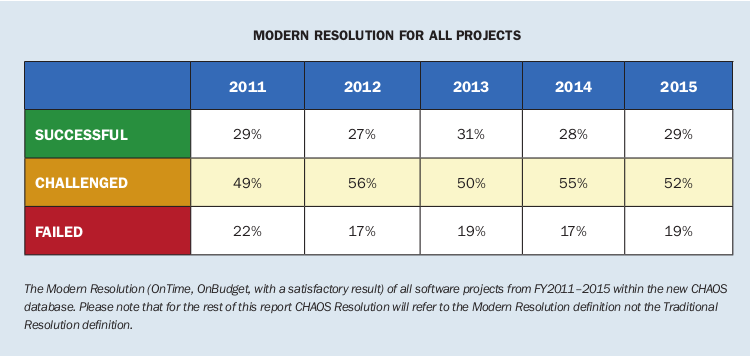
\includegraphics[width=0.9\linewidth]{modern2}
	\caption{Chaos report: �xito en proyectos de desarrollo. \cite{p1}}
\end{figure}


\end{frame}

	\begin{frame}
	\frametitle{La crisis del software}
	\begin{figure}
		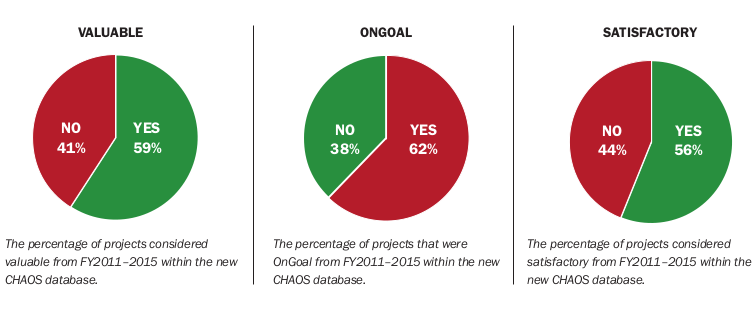
\includegraphics[width=0.9\linewidth]{modern1}
		\caption{Chaos report: resoluci�n moderna de proyectos de software. \cite{p1}}
	\end{figure}
	
	
\end{frame}

	\begin{frame}
	\frametitle{La crisis del software}
	Es interesante tambi�n analizar datos de los estudios de 2011 en cuanto a funcionalidad desarrollada y utilizada posteriormente en los proyectos de software:
	\begin{figure}
		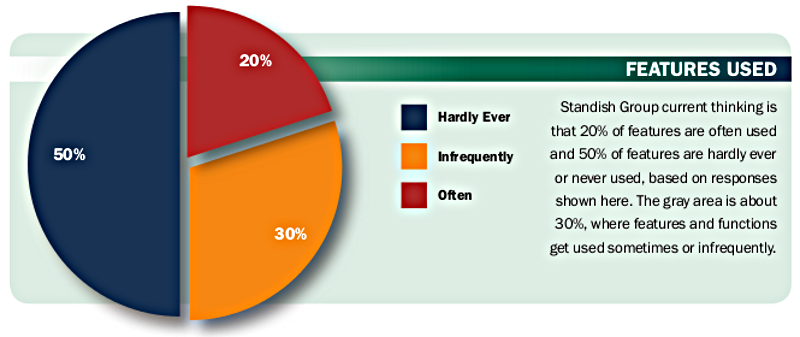
\includegraphics[width=0.9\linewidth]{features2011}
		\caption{Chaos report 2011: funcionalidad desarrollada utilizada en proyectos software.}
	\end{figure}
	
	
\end{frame}

	\begin{frame}
	\frametitle{Posibles causas}

	\begin{table}
	\begin{tabular}{l r}
		\toprule
		\textbf{Causa} & \textbf{\% del total} \\
		\midrule
		Falta de participaci�n de los usuarios 	& 12.8 \\
		Especificaciones poco claras o incompletas	& 12.3 \\
		Especificaciones cambiantes & 11.8 \\
		Falta de apoyo de la Direcci�n & 7.5 \\
		Falta de habilidades t�cnicas & 6.4 \\
		Otros &	50.2 \\
		\bottomrule
	\end{tabular}
	\caption{Causas de fracaso de los proyectos de software. Fuente: \cite{p4}}
\end{table}

	
\end{frame}

	\begin{frame}
	\frametitle{Otros datos}
	\begin{itemize}
	\item Estudio de defectos por categor�a encontr� que la m�s amplia era la de requisitos (41\%) \footnote{Fuente: \href{https://dl.acm.org/citation.cfm?id=625190}{Reliability Measurement from Theory to Practice , Sheldon, F., Kavi, K. et al.}}
	\item Estudios muestran que los requisitos son susceptibles de cambiar un 25\% o m�s \footnote{Fuente: \href{http://csse.usc.edu/TECHRPTS/1986/usccse86-501/usccse86-501.pdf}{Understanding and Controlling Software Costs , Boehm et al.}}
	\item Estudio con 38 organizaciones y 1027 proyectos: solo el 12,7\% tuvieron �xito y el factor con mayor contribuci�n para el fracaso fue el desarrollo en cascada, citado en el 82\% de los proyectos como causa principal del mismo, con una influencia global ponderada del 25\%.\footnote{Fuente: \href{https://archive.bcs.org/bulletin/jan00/article1.htm}{BCS Computer Bulletin, Thomas M.}}
	\end{itemize}
\begin{block}{Coste de correcci�n de defectos}
	\href{http://csse.usc.edu/TECHRPTS/1987/usccse87-503/usccse87-503.pdf}{Bohem} \cite{p5} mostr� que el coste de corregir un defecto se incrementa de manera no lineal a medida que transcurren las fases de un proyecto.
\end{block}
	
	
\end{frame}

	\begin{frame}
	\frametitle{La realidad del desarrollo de software}

	\begin{figure}
		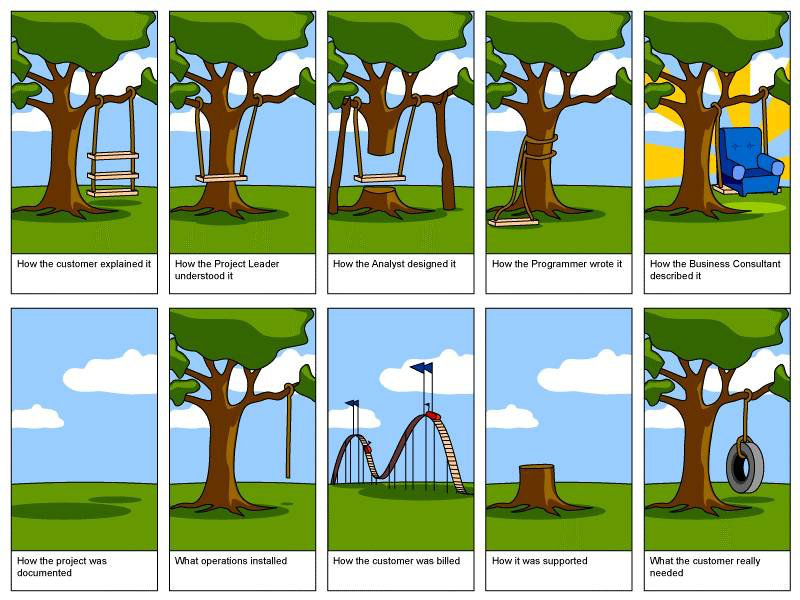
\includegraphics[width=0.9\linewidth]{req}
		\caption{La realidad del desarrollo de software.}
	\end{figure}
	
	
\end{frame}
	
	%------------------------------------------------
	
	\begin{frame}
		\frametitle{Referencias}
		\footnotesize{
			\begin{thebibliography}{99} % Beamer does not support BibTeX so references must be inserted manually as below
				\bibitem[Standish Group, 2015]{p1} The Standish Group (2015)
				\newblock Chaos Report 2015.
				
				\bibitem[Standish Group, 2014]{p4} The Standish Group (2014)
				\newblock Chaos Report White Paper 2014.
				
				\bibitem[Jorgensen, 2006]{p2} Jorgensen, M. y Molokken-Ostvod, K. (2006)
				\newblock How large are software cost overruns. A review of the 2004 CHAOS report.
				
				\bibitem[Laurenz, 2010]{p3} Eveleens, J. Laurenz and Verhoef, Chris. (2010)
				\newblock The Rise and Fall of the Chaos Report Figures.
				
				\bibitem[Bohem, 1987]{p5} Bohem, B. (1987)
				\newblock Industrial Software Metrics: a top-ten list.
			
				
			\end{thebibliography}
		}
	\end{frame}
	
	
	
	%------------------------------------------------
	
	
	%----------------------------------------------------------------------------------------
	
\end{document}